\section{Chapter 6: Static and Moving Patterns}
\graphicspath{ {pngs/ch6/} }

\secttoc

What is the best mapping from structured data to the display?
How can 2D space be divided into perceptually distinct regions?
Under what conditions are patterns perceived similar?
Visual connection between objects?
Mostly 2D, although some 3D properties are also important.
Pattern finding, hooray!


Visual system ranges from massively parallel primitive processing to high level
analysis of about one to five objects per fixation. Pattern perception is the
middle ground.


\begin{mdframed}\begin{multicols}{2}
    \subsection{Gestalt (pattern in German) Laws}
    A group of German psychologists in 1912 founded the Gestalt school of
    psychology.


    \begin{compactdesc}
        \item[Proximity] perceptual organization. Small spacing can have large
            effects. Consider spatial concentration and small size of fovea.
        \item[Similarity] similar elements should be grouped. Use channel theory
            and integral/separable dimensions. Good for independent patterns.
        \item[Connectedness] overlooked by originals. Connecting by lines.
        \item[Continuity] Smooth continuous objects are perceived better.
        \item[Symmetry] so good! Maybe for two time series? Important patterns
            must be small. 1 degree in width, 2 degrees in height centered at
            fovea. Don't make it too large. Horizontal/vertical is easier to
            see. Provide a frame of reference.
        \item[Closure and common region] Closed contours are seen as objects.
            Open ones are broken. Great for inside-outside divisions.
            Venn-Euler diagrams are used during introduction to set theory.
            Also used in window-based computer UIs.
        \item[Clarify closures] if they have a complicated shape with
            a Cornsweet edge, texture or color.
        \item[Figure-ground] figure is perceived in the foreground.
            Ground is everything ``behind'' it. Many Gestalt features help
            people segment (or not) an image. Closed contour, symmetry,
            amount of white area all contribute.
        \item[Relative size] smaller things are more object-like.
        \item[Rubin's Vase figure] high-level learned face recognition fights
            mid-level Gestalt figure detection processes.
        \item[Common fate] a motion based law discussed later.
        \item[More on Contours] continuous elongated boundaries between
            regions. Fundamental, receives much attention.
        \item[Randomly placed and oriented] Gabor patches. Continuity
            between patches with linear continuity is easiest to perceive.
            More wiggly patterns can also be detected.
        \item[Theory] inhibition between neurons with nonaligned receptive
            fields and mutual reinforcement between neurons with smoothly
            aligned patches. The winner take-all effect!
        \item[Controversial synchronous firing theory] neurons firing united
            may be how the brain retains higher-level patterns.
            Even if false, there is some neural mechanism enhancing contour
            detection.
    \end{compactdesc}
    \begin{figure}[H]
        \centering
        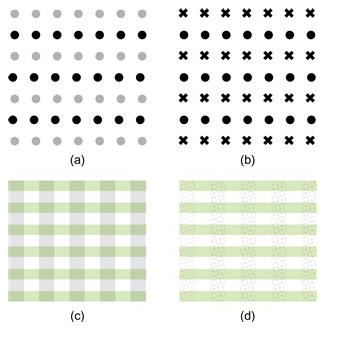
\includegraphics[width=0.2\textwidth]{Gestalten/similarity.png}
        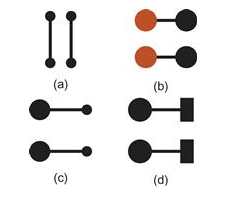
\includegraphics[width=0.2\textwidth]{Gestalten/connectedness.png}
        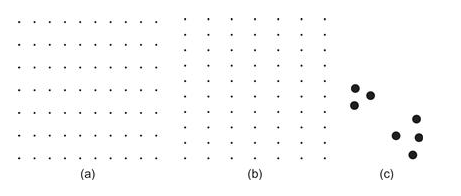
\includegraphics[width=0.2\textwidth]{Gestalten/proximity.png}
        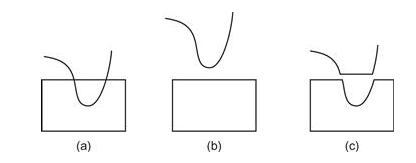
\includegraphics[width=0.2\textwidth]{Gestalten/continuity.png}
        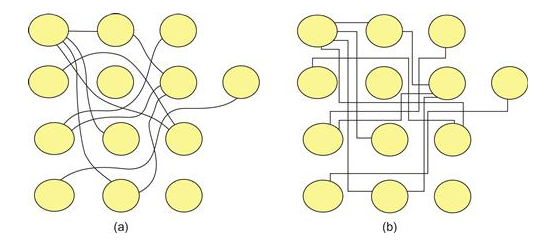
\includegraphics[width=0.2\textwidth]{Gestalten/continuity2.png}
        \caption{Similarity, connectedness, proximity, and continuity$\cdot2$}
    \end{figure}
    \begin{figure}[H]
        \centering
        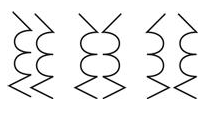
\includegraphics[width=0.1\textwidth]{Gestalten/symmetry.png}
        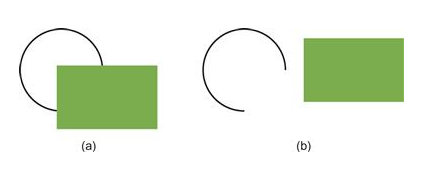
\includegraphics[width=0.15\textwidth]{Gestalten/closure.png}
        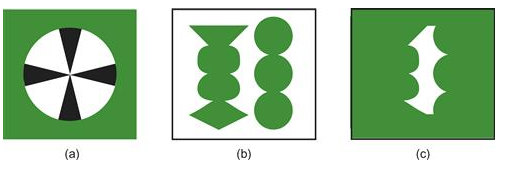
\includegraphics[width=0.15\textwidth]{Gestalten/figure_ground.png}
        \caption{Symmetry, closure, and figure and ground}
    \end{figure}
\end{multicols}\end{mdframed}

\begin{mdframed}
\begin{multicols}{2}
    \begin{figure}[H]
        \centering
        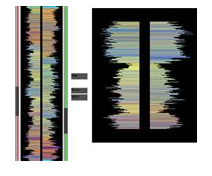
\includegraphics[width=0.4\textwidth]{symmetry_vis.png}
        \caption{Vis showing similarity in two time series using symmetry.}
    \end{figure}
    \begin{figure}[H]
        \centering
        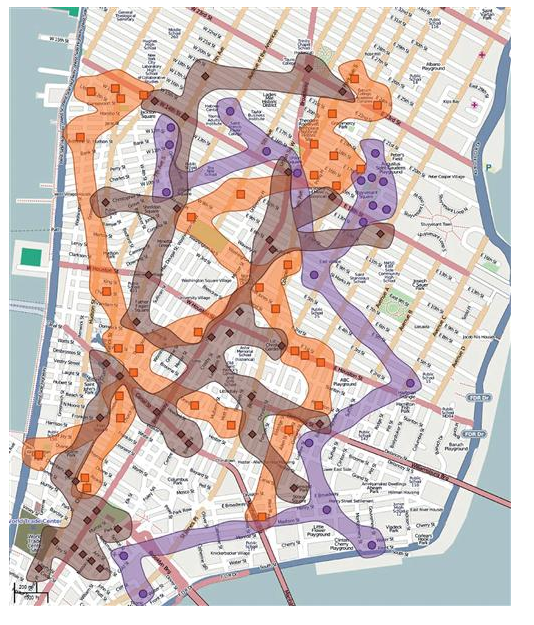
\includegraphics[width=0.3\textwidth]{color_and_region_vis.png}
        \caption{Contour, color and transparency to show distribution of
            hotels (orange), subway stations (brown), and medical clinic
            (purple).}
    \end{figure}
\end{multicols}
\end{mdframed}


\begin{mdframed}\begin{multicols}{2}
\subsection{Visualizing Vector Fields}
\begin{compactdesc}
    \item[Perceiving Orientation and direction] and magnitude.
    \item[Comparing 2D Flow Visualization techniques]
        A head to tail arrangement of vectors is ideal. Continuous contours
        provide the easiest perception of orientation, but do not show
        direction or magnitude. Randomly spaced, unconnected vectors are no
        good.
    \item[Tasks during flow visualization] are varied and depend on the
        application. Here are some:
        \begin{compactenum}
        \item Speed, orientation and direction at an arbitrary point
        \item Location and nature of critical points
        \item Advection trajectory
        \item High and low magnitude
        \item High and low curl
        \item High and low turbulence
        \end{compactenum}

    \item[Showing direction]
        Plain arrows produce clutter with their contours, their directional
        asymmetry
        is weak.
        It is better to use long narrow airfoils/pen-strokes.
        Can also vary gray level along the arrow. Called ``streamlets.''
        Stronger neural signal = more magnitude.

\end{compactdesc}
    \begin{figure}[H]
        \centering
        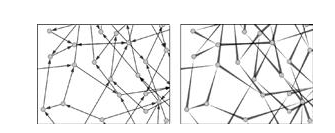
\includegraphics[width=0.25\textwidth]{link_vis.png}
        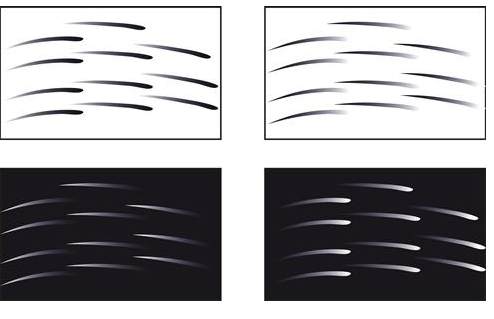
\includegraphics[width=0.2\textwidth]{streamlets.png}
        \caption{Left: two methods of drawing links, middle is more effective.
        Right: streamlets, effective for links}
    \end{figure}
    \begin{figure}[H]
        \centering
        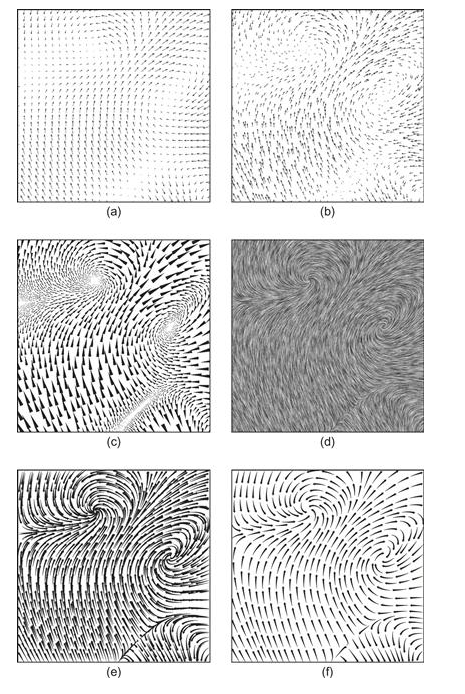
\includegraphics[width=0.6\linewidth]{six_flows.png}
        \caption{Six different vector field visualizations.
        Arrows a regular grid, arrows on a jittered
        grid to reduce perceptual aliasing, triangle icons with size
        indicating strength (density inversely related to size), line
        integral convolution, large-head arrows along a stream-line instead of
        a grid, large-head arrows along streamlines with constant spacing.}
    \end{figure}
\end{multicols}\end{mdframed}

\begin{mdframed}\begin{multicols}{2}
\subsection{Texture: Theory and Data Mapping}
    \begin{figure}[H]
        \centering
        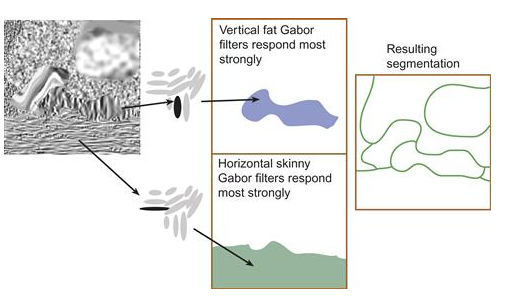
\includegraphics[width=\linewidth]{gabor_and_texture.png}
        \caption{Gabors can explain texture-based segmentation}
    \end{figure}

\begin{compactdesc}
    \item[Texture segmentation] regions defined by texture. Independent axis.
    \item[Gabor] is a Gaussian envelope * sine wave
    \item[Gabor filters] respond strongly to areas with dominant spatial
        frequencies and orientations. Contrast of textures is an independent
        feature.
    \item[Feature map] consisting of Gabors of different orientation can show
        primal sensitivity.
\end{compactdesc}

    \begin{figure}[H]
        \centering
        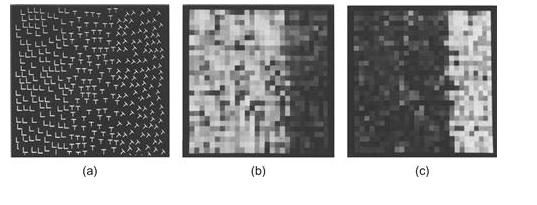
\includegraphics[width=0.7\linewidth]{gabors_and_classification.png}
        \caption{(a) Ts and Ls are difficult to segment, but the leaning Ts can
        be distinguished easily. (b) feature map of vertical gabors. (c)
        feature map of oblique gabors}
    \end{figure}

\end{multicols}\end{mdframed}



\begin{mdframed}\begin{multicols}{2}
\subsection{Information Density, An Uncertainty Principle}
\begin{compactdesc}
    \item[Perception of position, orientation, and size] are related
        by an uncertainty principle.
    \item[Orientation] can't use size as much
    \item[Size] less detail can be shown with larger elements
    \item[Gabors] can be stretched to specify either spatial frequency (size)
        or orientation more precisely.
    \item[Primary dimensions of texture]
        Real Gabors expose many variables, but in our visual systems Gabors
        with large Gaussians are coupled with high frequency cosine components
        and same goes for small and low frequencies. Thus a simpler three
        component model can be proposed:
        \\
        Orientation: cosine component
        \\
        Scale: $\frac{1}{spatial freq}$
        \\
        Contrast: Amplitude or contrast
    \item[Texture contrast effect] the same texture overlayed on another
        appears different. Some textures can interfere with other components,
        like lines.
    \item[Other dimensions] the world of texture is much richer than these
        three variables, though they are dominant. Randomness is also
        important.
    \item[Nominal coding] is the most common use for textures.
        Spatial frequencies should differ by a factor of 3, orientation
        by 30 degrees; where all other primitive factors are held constant.
\end{compactdesc}
    \begin{figure}[H]
        \centering
        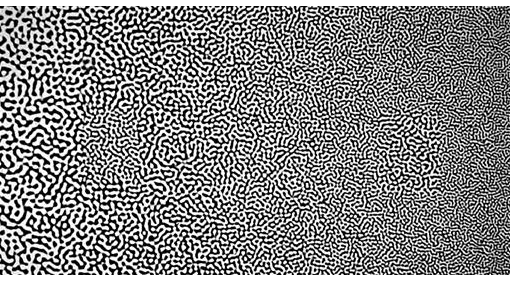
\includegraphics[width=0.4\textwidth]{texture_contrast.png}
        \caption{The texture contrast effect. The two patches on the left and
            right have the same granularity, but the texture contrast makes
            them seem different.}
    \end{figure}
\end{multicols}\end{mdframed}



\begin{mdframed}\begin{multicols}{2}
\subsubsection{Case studies and more texture}
\begin{compactdesc}
    \item[Univariate and multivariate Maps] Scalars: most common is to
        vary element size according to the value. Limited because
        elements must be small to accommodate the data.
    \item[Orientes sliver textures] for more than one scalar.
        Sliver contrast indicates magnitude, each dimension has its own sliver
        orientation. Not readable with many variables.
    \item[Attempt two:] glyph color (temperature), orientation and direction
        (wind), glyph area coverage (wind speed), density of elements
        (pressure).
    \item[3, a Scientist and designer:] cross-section of a mouse spinal column.
        Shows 7 variables at each location. Tradeoffs. Glyphs are textured,
        and end up camouflaged. Worsened by texture orientation.
        Luminance has the highest range, all other components cause noise and
        distract from detail.
    \item[Quantitative texture sequence 1] 10-step texture steps and color.
        Textures gain luminance. Two maps are successfully combined.
    \item[Quantitative texture sequence 2] 14-step texture (different shapes,
        contrast) steps, color, animated streamlet vector field, number labels
        and a map of the Northwestern USA.
        Amen! Will need training.
    \item[Texture is most valuable] if there are two scalar values.
        To be reasonable, it consumes some luminance channel.
\end{compactdesc}
\end{multicols}\end{mdframed}

\begin{mdframed}\begin{multicols}{4}
    \begin{figure}[H]
        \centering
        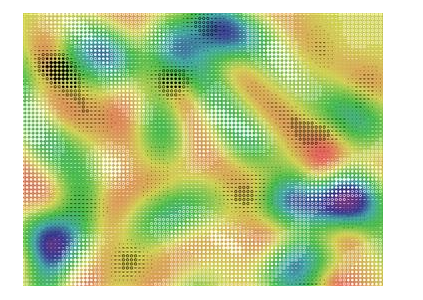
\includegraphics[width=0.2\textwidth]{color_and_texture_vis.png}
        \caption{Bivariate map, color and a carefully designed texture sequence}
    \end{figure}
    \begin{figure}[H]
        \centering
        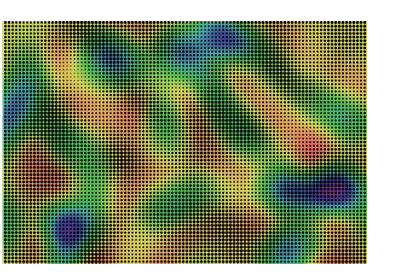
\includegraphics[width=0.2\textwidth]{color_and_size_vis.png}
        \caption{Bivariate map, color and texture element.}
    \end{figure}
    \begin{figure}[H]
        \centering
        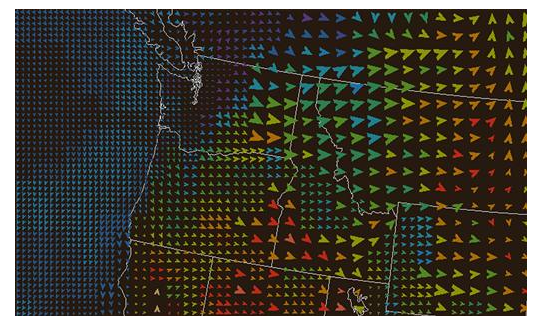
\includegraphics[width=0.2\textwidth]{weather1_vis.png}
        \caption{Wind orientation and direction mapped to glyph rotation. Wind
        speed to glyph area. Pressure is density. Temperature is color.}
    \end{figure}
    \begin{figure}[H]
        \centering
        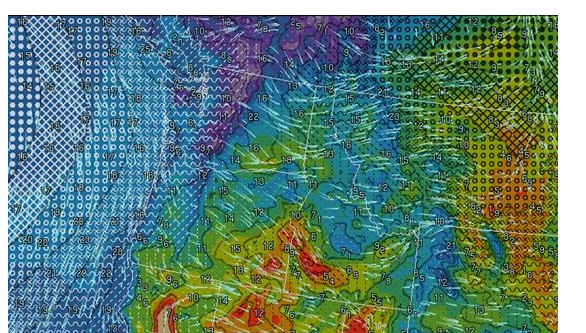
\includegraphics[width=0.2\textwidth]{weather_texture_vis.png}
        \caption{Temperature is color, pressure is a sequence of 14 textures,
        wind orientation and direction are animated streamlets, wind speed is
    animation speed and numbers.}
    \end{figure}

\end{multicols}\end{mdframed}



\begin{mdframed}\begin{multicols}{2}
\subsection{Perception of transparency}
\begin{compactdesc}
    \item[Different layers at the same time] common in GIS. The layers
        will always interfere with each other.
    \item[Continuity and color] relationships are the most important!
    \item[Took longer] to read from menu with text or wireframe images
        as background than one with smoothly shaded images as background.
    \item[Laciness] as opposed to a single fused image, view each layer through
        a screen pattern. The effect can be bistable. Asks for tuning because
        of perceptual interference.
    \item[Luminance contrast] is needed with texture layered over color-coded
        data. This constrains the color palette.
\end{compactdesc}
\end{multicols}\end{mdframed}



\begin{mdframed}\begin{multicols}{2}
\subsection{Perceiving Patterns in Multidimensional Discrete Data}
\begin{compactdesc}
    \item[LOTS OF MONEY] advertisements and demographics.
    \item[Tabulated data] is hard to read.
    \item[Three dimensions:] common to use point size or color or oscillatory
        motion along with 2D position.
\end{compactdesc}


\subsubsection{Higher dimensions}
\begin{compactdesc}
    \item[Draw 2D graphs] of each possible pairing. Difficult to see higher
        dimensional relationsips.
    \item[Parallel coordinates plot] each attribute is a vertical line,
        a ``point'' of data is represented by a sequence of lines connecting
        various vertical ones.
    \item[PC plots depend on order] of vertical bars, thus it is useful to
        randomize order and then explore.
    \item[PC plots with scatter plots] embedded are more useful than
        draftsman's.
    \item[meant to be interactive] via ``brushing,'' highlighting the polylines
        passing through a range.
    \item[5D] scatter plot, red, green and blue. Color dimensions could be
        as effective as spatial dimensions when looking for clusters.
    \item[Interpreting] these clusters can be hard. Greenish = low on red
        or high in green?
    \item[Color can improve PC plots] by painting with algorithmially
        determined color-density schemes.
\end{compactdesc}

    \begin{figure}[H]
        \centering
        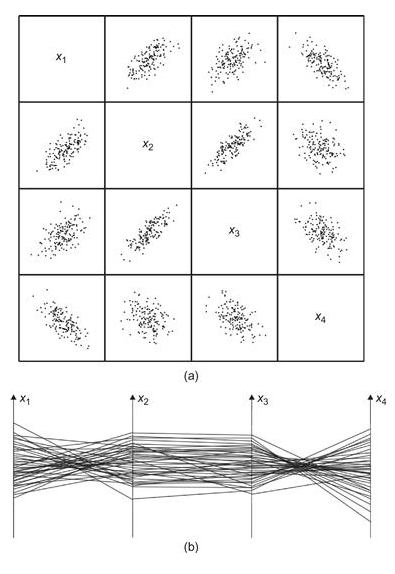
\includegraphics[width=0.4\textwidth]{multivariate_vis.png}
        \caption{(a) generalized draftsman's plot. (b) parallel coordinates
        plot.}
    \end{figure}

\end{multicols}\end{mdframed}



\begin{mdframed}\begin{multicols}{2}
\subsection{Pattern learning}
\begin{compactdesc}
    \item[Low-level features] can't be improved much.
    \item[Intermediate complexity] some learning can occur
    \item[Higher-level] high level of learning displayed!
    \item[Biased experiments] a person has seen millions of letters, it
        would be difficult to improve on that skill. Logarithmic relationship.
    \item[Priming] transient effects, last minutes to days. Ability to
        detect certain patterns is improved. It could be visual learning or
        something less.
    \item[Show examples ahead of time]
    \item[Standards] should be relied upon. If your audience has learned
        certain patterns, use them.
\end{compactdesc}

\subsubsection{Vigilance}
\begin{compactdesc}
    \item[Some notes] about vigilance:
    \begin{compactenum}
        \item Performance falls after the first hour.
        \item Fatigue is negative
        \item Difficult task requires a high level of sustained attention.
            No multi tasking.
        \item Irrelevant signals are negative
        \item Twice as likely to see frequent targets than rare ones.
    \end{compactenum}
    \item[Can be improved by] offering some extra information:
    \begin{compactenum}
        \item target reminders at frequent intervals. Important if
            many targets.
        \item use people's sensitivity to motion
        \item the signal must be made as distinct as possible
        \item in-place retraining sessions help (bursts of frequent targets)
    \end{compactenum}

\end{compactdesc}
\end{multicols}\end{mdframed}



\begin{mdframed}\begin{multicols}{2}
\subsection{Visual grammar of node-link diagrams}
\begin{compactdesc}
    \item[Graph drawing] academic field dedicated to readable graphs.
        Minimize link crossings, structure symmetry, minimal bends in links.
    \item[Will analyze] node-link diagrams, broader concepth than graphs.
    \item[Fundamental argument:] closed contours are easily perceived as
        objects. Our sensory perception provides a scaffolding for even our
        most abstract concepts.
    \item[Interpretations of a countour:] ring, flat disk, ball, hole,
        boundary between two objects (disk in a hole). Convention, context
        and any Gestalt tell us which is correct.
    \item[Closed contour] object or entity
    \item[Compact shapes] entity types
    \item[Color of region] entity types
    \item[Size of region] value, larger=more
    \item[Majority of diagrams] are simple. No variance in shape, size or color.
        Can show structure but not entity type.
    \item[A more varied] visual grammar:

    \item[Streamlets] work good as asymmetric connectors

\end{compactdesc}

\subsection{Visual grammar of node-link diagrams}
\begin{compactdesc}
    \item[Three graphical marks] are common to all maps: areas, line features,
        small symbols.

    \item[Treemap] represents tree's leafs. Leafs of lower depth are given
        more area.
    \item[Similar for maps] closed contours, colored/textured regions,
        lines, dots, dot on line, dot in region, line crossing region, line
        exits region, overlapping regions.
\end{compactdesc}

    \begin{figure}[H]
        \centering
        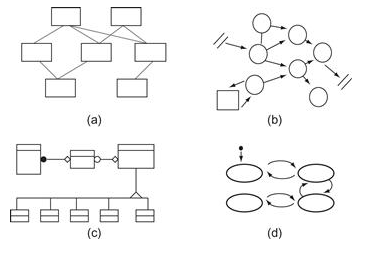
\includegraphics[width=0.4\textwidth]{node_link_vis.png}
        \caption{Several node-link diagrams used in software engineering.}
    \end{figure}
    \begin{figure}[H]
        \centering
        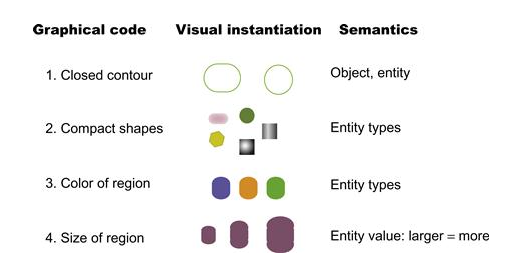
\includegraphics[width=0.4\textwidth]{node_link_grammar.png}
        \caption{Grammar of a node link visualization.}
    \end{figure}

\end{multicols}
\end{mdframed}


\begin{mdframed}\begin{multicols}{2}
\subsection{Patterns in motion}
\begin{compactdesc}
    \item[Pattern detection in motions] is not as well understood as other
        pattern detection systems.
    \item[Correspondence problem] identical objects may be confused for
        each other in frames of animation. If the distance between all
        elements is $\lambda$ we are limited to a maximum displacement of
        $\lambda / 2$ on each frame.
    \item[Wagon-wheel effect] they seem to rotate backwards! To show
        direction, the maximum change per frame should be $\lambda / 3$.
    \item[60 FPS] gives 20 messages per second.
    \item[Can be fixed] by giving objects different looks. The limit is more
        like $3 \lambda$, or 180 messages per second.
\end{compactdesc}
    \subsubsection{Form and contour in motion}
\begin{compactdesc}
    \item[Relative motion:] very sensitive
    \item[Motion is an attribute] like color or shape.
    \item[Phase of motion] is perceived best. Comparable to point size or
        gray value.
    \item[elliptical motion] can help segment nodes into groups
    \item[Moving frames] a rectangular frame provides a strong contextual
        cue for motion perception. A bright frame moved around a bright dot,
        the static dot seemed to move.
    \item[hierarchy] the brain groups moving objects in a hierarchy
    \item[sensitive] to 0.5cm to 4cm per second.
    \item[rectangular frames] can help highlight local relative motion
\end{compactdesc}

\begin{compactdesc}
    \item[expressive motion,] motion can express more subtle phenomena
    \item[perception of causality] elements launch, entrain, trigger
        other elements. Precise timing is required.
        Launching occurs within 70ms, delayed launching up to 160ms, after
        this no causality is perceived.
    \item[motion with a biological] origin can be detected given the slightest
        of hints. Random-seeming collection of dots, once animated, became
        people with gender performing specific tasks. Kindness, fear and
        aggression can be expressed.
    \item[animation] can easily expand the information perceived from a
        diagram.
\end{compactdesc}
\end{multicols}\end{mdframed}


\begin{mdframed}\begin{multicols}{2}
\subsection{Processes of Pattern Finding}
\begin{compactdesc}
    \item[we see what we know] but the process of detecting novel patterns
        is more difficult.
    \item[tasks encourage] tuning of visual queries. If color is where
        information lies, then color will be analyzed more thoroughly.
    \item[Only a small] number of contours can be traced
    \item[Attentional shrouds] regions of different texture compete
        for attention. Visual queries allocate attention.
    \item[Beyond a certain complexity] novel patterns cannot be easily
        grasped.
\end{compactdesc}
\begin{figure}[H]
\centering
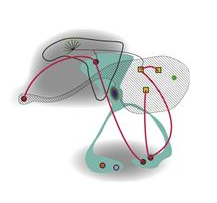
\includegraphics[width=0.2\textwidth]{pattern_vis.png}
\caption{Attend to different components, feel others fade.}
\end{figure}
\end{multicols}\end{mdframed}




